%%%%%%%%%%%%%%%%%%%%%%%%%%%%%%
% Ioannis Petrousov
% petrousov@gmail.com
% 2016
%
% Custom Latex thesis template
% to be used for Greek language.
%
% Initial compile:
%	1. xelatex
%	2. bibtex
%	3. xelatex
%	4. xelatex
%
% Further compile:
%
% A: If you change the biblipgraphy file
%	1. biblatex
%	2. xelatex
%	3. xelatex
%
% B: If you DONT change the biblipgraphy file
%	1. xelatex
%	2. xelatex
%%%%%%%%%%%%%%%%%%%%%%%%%%%%%%

% Use the following documentclass declaration if you plan to make a hardcopy
% The twoside option shift text for making a book print
%\documentclass[12pt,twoside]{report}

% Use the following documentclass for PDF and to view on computer only
\documentclass[12pt,a4paper]{report}%{book}

% xelatex wants fontspec
\usepackage{fontspec}
\usepackage{xltxtra}
\usepackage{xgreek}
\setmainfont[Mapping=tex-text]{GFS Didot}
\usepackage{graphicx}
% put images in images path
\graphicspath{{images/}}
\usepackage{setspace}

% use this package to define custom colors
\usepackage{xcolor}

% create colors
\colorlet{punct}{red!60!black}
\definecolor{background}{HTML}{EEEEEE}
\definecolor{delim}{RGB}{20,105,176}
\colorlet{numb}{magenta!60!black}

% use this package for algorithms
\usepackage{algorithm2e}

% use this package to show actual code listings
\usepackage{listings}

% change listings name in caption to Απεικόνιση
\renewcommand{\lstlistingname}{Απεικόνιση}

% change listings name in contents page to Κατάλογος απεικονήσεων
\renewcommand\lstlistlistingname{Κατάλογος απεικονίσεων}

% set custom colorscheme for listings with language=lang1 to make them stand out more
% http://tex.stackexchange.com/questions/83085/how-to-improve-listings-display-of-json-files
\lstdefinelanguage{lang1}{
    basicstyle=\normalfont\ttfamily,
%    numbers=left,
%    numberstyle=\scriptsize,
%    stepnumber=1,
%    numbersep=8pt,
    showstringspaces=false,
    breaklines=true,
    frame=lines,
    backgroundcolor=\color{background},
    literate=
     *{0}{{{\color{numb}0}}}{1}
      {1}{{{\color{numb}1}}}{1}
      {2}{{{\color{numb}2}}}{1}
      {3}{{{\color{numb}3}}}{1}
      {4}{{{\color{numb}4}}}{1}
      {5}{{{\color{numb}5}}}{1}
      {6}{{{\color{numb}6}}}{1}
      {7}{{{\color{numb}7}}}{1}
      {8}{{{\color{numb}8}}}{1}
      {9}{{{\color{numb}9}}}{1}
      {:}{{{\color{punct}{:}}}}{1}
      {,}{{{\color{punct}{,}}}}{1}
      {\{}{{{\color{delim}{\{}}}}{1}
      {\}}{{{\color{delim}{\}}}}}{1}
      {[}{{{\color{delim}{[}}}}{1}
      {]}{{{\color{delim}{]}}}}{1},
}


% create command for blank page
\usepackage{afterpage}
\newcommand\blankpage{%
    \null
    \thispagestyle{empty}%
    \addtocounter{page}{-1}%
    \newpage}

% add clickable hyperlinks
\usepackage{hyperref}
\hypersetup{
    colorlinks,
    citecolor=black,
    filecolor=black,
    linkcolor=black,
    urlcolor=black
}

% use fancy header and footer
\usepackage{fancyhdr}
\usepackage{blindtext} % to quickly get a full document

% Turn on the style
\pagestyle{fancy}

% Clear the header and footer
\fancyhf{}

% Set the right side of the footer to be the page number
\fancyfoot[R]{\thepage}

% set page number appearance to bottom right
\fancypagestyle{plain}{%
    \renewcommand{\headrulewidth}{0pt}
    \fancyhf{}
    \fancyfoot[R]{\thepage}%
}

% chapter appearance format
\usepackage{titlesec}
\titleformat{\chapter}[display]
{\bfseries\huge}{\chaptertitlename\space\thechapter}{16pt}{}

% section appearance format
\titleformat{\section}
{\bfseries\normalfont\large}{\thesection}{14pt}{}

% subsection appearance format
\titleformat{\subsection}
{\normalfont}{\thesubsection}{12pt}{}

\newcommand{\HRule}{\rule{\linewidth}{0.5mm}}

% change the word 'Alrogithm' in caption to Αλγόριθμος
\renewcommand*{\algorithmcfname}{Αλγόριθμος}

% Change "List of Algorithms" to "Κατάλογος αλγορίθμων"
\renewcommand\listalgorithmcfname{Κατάλογος αλγορίθμων}

\begin{document}
\begin{titlepage}
\begin{center}
\begin{figure}[h]
\centering 
\includegraphics{icte.png}
\end{figure}
{\LARGE Πανεπιστήμιο Δυτικής 
Μακεδονίας\\}
{\Large Τμήμα Μηχανικών Πληροφορικής \&
Τηλεπικοινωνιών \\}

\begin{center}
% leave 2 cm from above text
\vspace{2cm}

\HRule \\[0.4cm]
{\huge Τίτλος διπλωματικής\\}
\HRule \\[0.4cm]
\end{center}

% put this on the bottom
\vfill
\begin{doublespacing}

{\LARGE 
Ιωάννης Πετρουσόβ\\}
{\Large Επιβλέπων Καθηγητής : Δρ. Μηνάς Δασυγένης\\}
\textbf{\Large Εργαστήριο Ψηφιακών Συστημάτων και Αρχιτεκτονικής Υπολογιστών}
\vfill 
{\Large \today}
\end{doublespacing}
\end{center}
\end{titlepage}

% insert blank page after title page
\afterpage{\blankpage}


\newpage
\chapter*{Περίληψη}
Περίληψη στα Ελληνικά...




% put this on the bottom
\vfill
\textbf{Λέξεις κλειδιά}: Python, FPGA, GHDL, ASIC, Cython




%\newpage
\chapter*{Abstract}
Abstract in English...

% put this on the bottom
\vfill
\textbf{Keywords}: Python, FPGA, GHDL, ASIC, Cython

% Insert copyright
\chapter*{Δήλωση Πνευματικών Δικαιωμάτων}

\noindent{Copyright (C) Ιωάννης Πετρουσόβ \& Μηνάς Δασυγένης, 2016, Κοζάνη}

% put this on bottom
\vfill
Υπογραφή Φοιτητή

%%%%%%

% insert table of contents
\newpage\tableofcontents

% insert list of figures
\listoffigures
\clearpage

% insert list of algorithms
\listofalgorithms
\clearpage

% insert list of tables
\listoftables
\clearpage

% insert list of listings
\lstlistoflistings
\clearpage

% leave blank page before main part
\blankpage

\chapter{Εισαγωγή}
\section{Ορισμός του προβλήματος}
Ορισμός του προβλήματος...


\section{Κίνητρα και Στόχοι Υλοποίησης}
Κίνητρα...


\section{Περιπτώσεις παρόμοιων εργαλείων}
Παρόμοιο έργο...

\section{Διάρθρωση κειμένου}
Τα υπόλοιπα κεφάλαια οργανώνονται ως εξής...

\chapter{Παραδείγματα}
Αυτή είναι μία παράγραφος...

Αυτή είναι μία άλλη παράγραφος...

\section{Παράδειγμα σχήματος}
Στην σχήμα \ref{fig:fpga_board_example}

\begin{figure}[h!]
\caption{Παράδειγμα μιας πλακέτα FPGA}
\centering
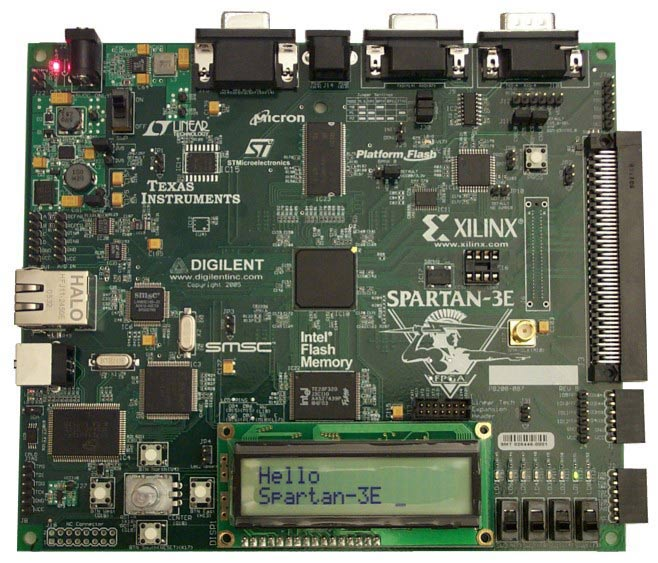
\includegraphics[scale=0.3]{fpga_board_example}
\label{fig:fpga_board_example}
\end{figure}

\section{Παράδειγμα υποσημείωσης}
Το ASIC \footnote{\url{http://www.pcmag.com/encyclopedia/term/38030/asic}} (application-specific integrated circuit)...

\section{Παράδειγμα αναφοράς}
H Python είναι μια γενικού σκοπού υψηλού επιπέδου γλώσσα προγραμματισμού \cite{van2007python}.



\section{Διαχωρισμός τμημάτων}
Αυτό είναι τμήμα

\subsection{Υποτμήμα}
Αυτό είναι υποτμήμα...

\section{Σύνοψη Κεφαλαίου}
Στο κεφάλαιο αυτό...

\chapter{Θεωρητικό μέρος}

\section{Παράδειγμα απεικόνισης}
Ένα ενδεικτικό παράδειγμα \ref{lst:listings_example}.

\begin{lstlisting}[label=lst:listings_example,caption=Παράδειγμα απεικόνισης]
{
	"function": ( (in0 + in1 ) * ( in2 + in3 ) )",
	"in0": 2,
	"in1": 2,
	"in2": 5,
	"in3": 5	
}
\end{lstlisting}


\section{Παράδειγμα πίνακα}
Στον πίνακα \ref{tbl:table_example} φαίνεται...

\begin{table}[h]
\centering
\caption{Επεξήγηση πίνακα}
\label{tbl:table_example}
\begin{tabular}{rcl}
(x,y,z)      & : & συντεταγμένες στοιχείου εισόδου    \\
outputport   & : & θύρα εξόδου προηγούμενου στοιχείου \\
(lsb,msb)    & : & εύρος bit εισόδου                  \\
signaltype   & : & τύπος σήματος (bit, stream)        \\
output\_port & : & αριθμός θύρας εξόδου              
\end{tabular}
\end{table}

\subsection{Παράδειγμα παραγράφου}

\paragraph{Αρχικά}
Στο πρώτο βήμα...


\paragraph{Ύστερα}
Στο δεύτερο βήμα...

\paragraph{Τελικά}
Στο τρίτο βήμα...

\chapter{Το λογισμικό μέρους}

\section{Παράδειγμα αλγόριθμου}
Στο \ref{alg:reverse_traversal} δίνεται ο αλγόριθμος που...

\begin{algorithm}[h!]
\SetAlgoLined
\label{alg:reverse_traversal}
\KwResult{stack}
 $theStack = create\_empty\_stack()$\;
 $theQueue = create\_empty\_queue()$\;
 $theQueue.enqueue(root\_node)$\;
 \While{theQueue is not empty}{
  $root = theQueue.dequeue()$\;
  \uIf{root.RightChild == +,-,*,/,)}{
  \tcp*[h]{case 1}\\
   $theQueue.enqueue(root.RightChild)$\;
   }
  \uIf{root.LeftChild == +,-,*,/,)}{
  \tcp*[h]{case 2}\\
   $theQueue.enqueue(root.LeftChild)$\;
   }
   theStack.push(root)
 }
 \caption{Αλγόριθμος επιστροφής στοίβας κόμβων δέντρου.}
\end{algorithm}


\section{Παράδειγμα αριθμητικής συνάρτησης}
Η συνάρτηση $f(x,y)=((2*x)+y)$ έχει...



\section{Παράδειγμα μεγάλου πίνακα}
Στον πίνακα \ref{tbl:code_files_metrics} δίνονται ορισμένες μετρικές

\begin{table}[!htbp]
\centering
\caption{Μετρικές αρχείων κώδικα.}
\label{tbl:code_files_metrics}
\begin{tabular}{|l|cccc|}
\hline
\multicolumn{1}{|c|}{\textbf{Language}} & \textbf{files} & \textbf{blank} & \textbf{comment} & \textbf{code} \\
Python                                  & 71             & 6445           & 8300             & 408377        \\
C                                       & 3              & 295            & 766              & 5850          \\
Bourne Shell                            & 14             & 195            & 154              & 561           \\
Cython                                  & 2              & 44             & 46               & 119           \\ \hline
\textbf{SUM}                            & 90             & 6979           & 9266             & 414907        \\ \hline
\end{tabular}
\end{table}

Βλέπουμε ότι το 98,42\% των περιεχομένων των αρχείων είναι\\
Python.

\section{Παράδειγμα απεικόνισης χωρίς σπάσιμο}
Η απεικόνιση \ref{lst:good_comment} δεν σπάει σε διαφορετικές σελίδες.
Αντίθετα, μεταφέρεται αυτούσια σε άδεια σελίδα.

\noindent\begin{minipage}{\linewidth}
\begin{lstlisting}[language=lang1,label=lst:good_comment,
caption=Διατήρηση απεικόνισης στην ίδια σελίδα.]
"""
This function will try to dynamically import
the requested module item from the module's
path.
If the module item does not exist, it will
call the function that creates it and import
it after it has been created.
INPUT:
    module_path [str] : full path of the
    module you want to import [a pathname
    with __init__.py inside]
    module_item  [str] : a *.py file
    inside the module path
OUTPUT:
    returns the handler for the requested
    module item.
    You can call the
    module_item.function()
"""
\end{lstlisting}
\end{minipage}


\bibliographystyle{plain}

{\footnotesize
\bibliography{refs}}
\end{document} 